\documentclass[]{article}
\usepackage{caption,subcaption,graphicx,float,url,amsmath,amssymb,tocloft}
\usepackage[hidelinks]{hyperref}
\usepackage[toc,acronym,nonumberlist]{glossaries}
\setacronymstyle{long-short}
\usepackage{glossaries-extra}
\graphicspath{{figs/}}
\setlength{\cftsubsecindent}{0em}
\setlength{\cftsecnumwidth}{3em}
\setlength{\cftsubsecnumwidth}{3em} 
%opening
\title{Notes from Origins of Life\\Week4: Early Life}
\author{Simon Crase}

\makeglossaries

\loadglsentries{glossary-entries}

\renewcommand{\thesection}{4.\arabic{section}}
\renewcommand{\glstextformat}[1]{\textbf{\em #1}}

\begin{document}

\maketitle

\begin{abstract}
   These are my notes from the $4^{th}$ week of the Santa Fe Institute Origins of Life Course\cite{sfi2019}. The course aims to push the field of Origins of Life research forward by bringing new and synthetic thinking to the question of how life emerged from an abiotic world.\\
   The content and images contained herein are the intellectual property of the Santa Fe Institute, with the exception of any errors in transcription, which are my own.
   These notes are distributed in the hope that they will be useful,
   but without any warranty, and without even the implied warranty of
   merchantability or fitness for a particular purpose. All feedback is welcome,
   but I don't necessarily undertake to do anything with it.
\end{abstract}

\setcounter{tocdepth}{2}
\tableofcontents
\listoffigures
\section{Introduction}

Lecturer: Chris Kempes


We'll discuss evolution in a pre-cellular world, chemical signatures of early life, protocells, and what the \gls{gls:LUCA} might have looked like.

\section{Protocells}

Lecturer: Sarah Mauer

We'll look at Protocells as a model for the origins of life. Aggregates are important for the origins of life--Figure \ref{fig:ImportanceOfAggregation}.

\begin{itemize}
	\item  Co-localize metabolic/genetic components
	\item   Define the individual to allow for 	selection
	\item   Direct involvement in metabolism
	\begin{itemize}
		\item 	Chemical gradients
		\item   Electron transfer reactions
		\item   Catalytic
	\end{itemize}
	\item   Protect metabolic/genetic 	components
\end{itemize}

\begin{figure}[H]
	\caption{Importance of aggregates to origins of life}\label{fig:ImportanceOfAggregation}
	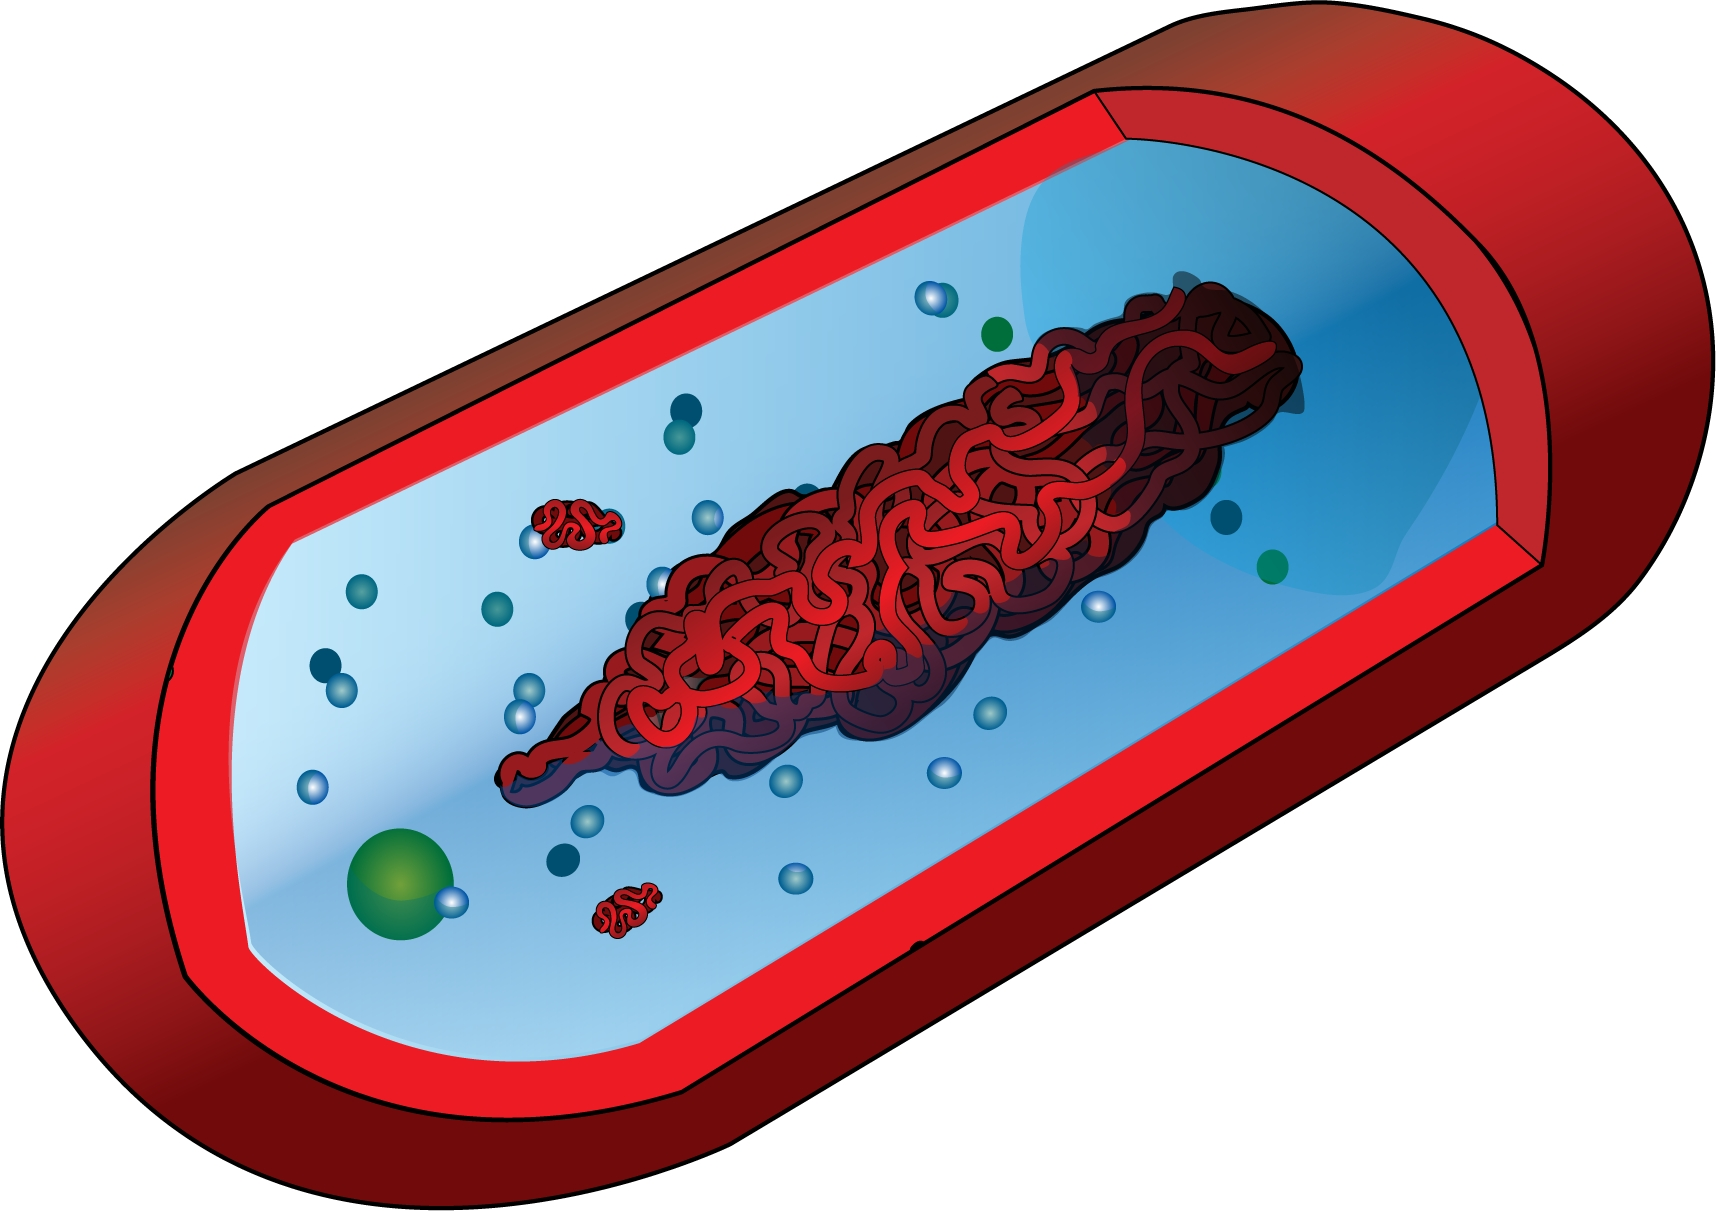
\includegraphics[width=0.9\textwidth]{ImportanceOfAggregation}
\end{figure}

See  \cite{deamer2017role},\cite{maurer2011primitive}, \cite{segre2001lipid}

Self-assembled structures

Controlled by the hydrophobic effect (entropy) and non-bonding interactions (e.g., hydrogen bonds)

\begin{table}[H]
	\caption{Aggregates that are used to model the origins of life}
	\begin{tabular}{l|p{4cm}|p{3cm}} \hline
		Type & Definition &Biological example\\ \hline
		Vesicle (Liposome)& Bilayer-enclosed aqueous compartment& Cells, membrane bound organelles,\\ \hline
		Oil droplet&
		Nonpolar bulk phase often stabilized by
		amphiphiles&
		Lipoproteins (LDL)\\ \hline
		Coacervate&
		\glsdesc{gls:coacervate}&
		P-bodies, membrane-less organelles\\ \hline
		Inorganic&&Thin films or crystals\\ \hline
	\end{tabular}
\end{table}


\begin{figure}[H]
	\centering
	\caption{Self-assembled structures}
	\label{fig:self-assembled-structures}
	\begin{subfigure}[b]{0.3\textwidth}
		\centering
		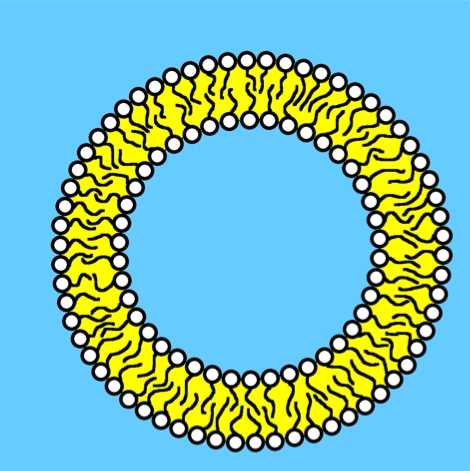
\includegraphics[width=\textwidth]{SelfAssembled1}
		\caption{Water}
		\label{fig:water}
	\end{subfigure}
	\hfill
	\begin{subfigure}[b]{0.3\textwidth}
		\centering
		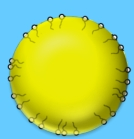
\includegraphics[width=\textwidth]{SelfAssembled2}
		\caption{Not water}
		\label{fig:not-water}
	\end{subfigure}
	\hfill
	\begin{subfigure}[b]{0.3\textwidth}
		\centering
		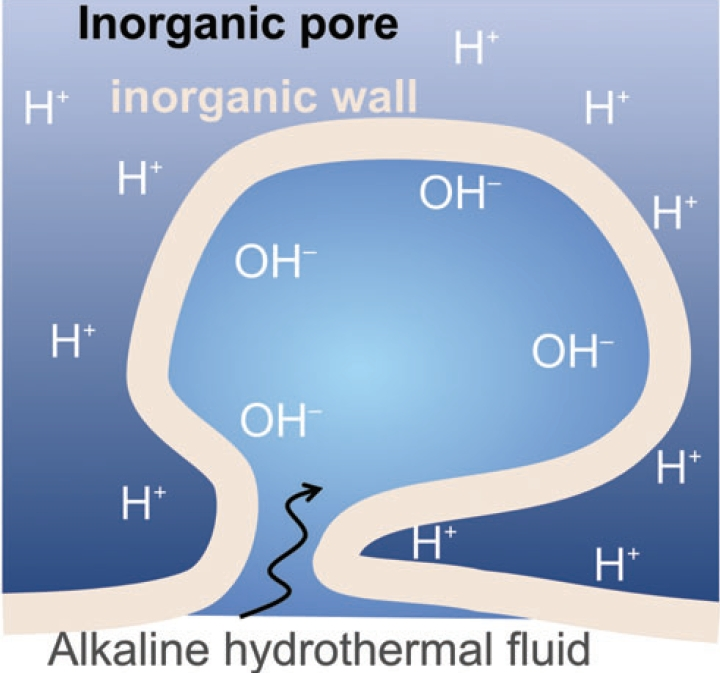
\includegraphics[width=\textwidth]{SelfAssembled3}
		\caption{Proton Gradient across thin inorganic barrier}
		\label{fig:proton-gradient}
	\end{subfigure}

\end{figure}

See \cite{sojo2016origin}

Factors that affect aggregation:
\begin{itemize}
	\item concentration;
	\item temperature;
	\item ionic strength;
	\item pH.
\end{itemize}

What chemistries do protocells harbour? Figure \ref{fig:ProtocellsAndReactions1} shows several possibilities:
\begin{itemize}
	\item A molecules interact with surface of aggregate through electrostatic interactions or hydrogen bonding;
	\item B hydrophobic effect sequestering non-polar molecule;
	\item C amphiphillic molecule anchored in membrane; 
	\item D molecule sequestered but still in water phase.
\end{itemize}

\begin{figure}[H]
	\caption{Aggregates interacting with molecules that are going to start life}\label{fig:ProtocellsAndReactions1}
	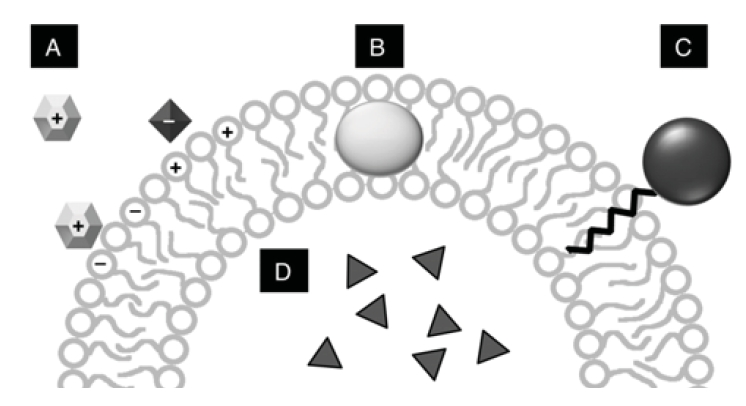
\includegraphics[width=0.9\textwidth]{ProtocellsAndReactions1}
\end{figure}

Figure \ref{fig:ProtocellsAndReactions2} depicts two locations for reactions.
\begin{itemize}
	\item A Surface associated reaction. Substrate becomes Product + Waste, and Waster drifts away. 
	\item B Catalytic network inside membrane, so we need to get rid of Waste.
\end{itemize}
\begin{figure}[H]
	\caption{Two locations for reactions}\label{fig:ProtocellsAndReactions2}
	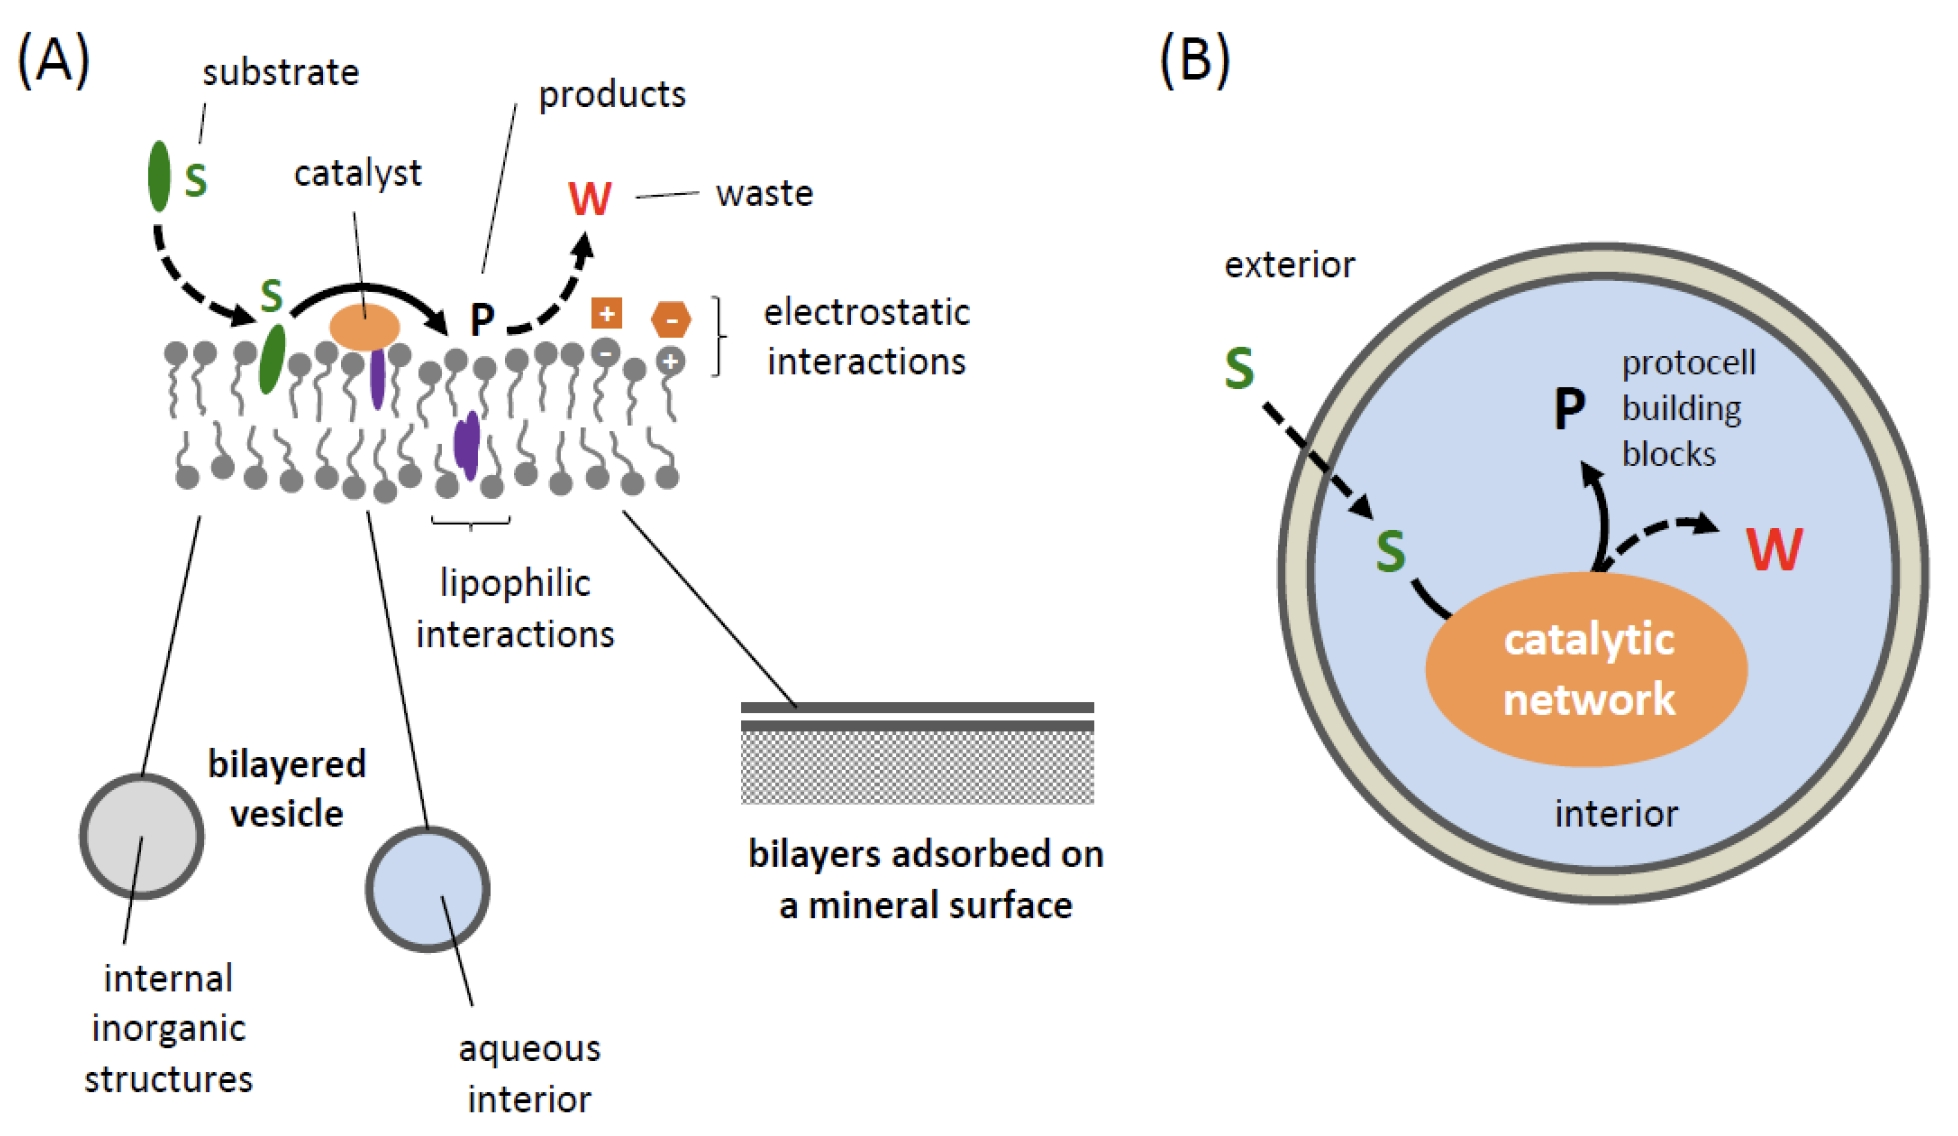
\includegraphics[width=0.9\textwidth]{ProtocellsAndReactions2}
\end{figure}

Figure \ref{fig:ProtocellsAndReactions3} shows an example of a reaction:  the Hammerhead ribosome can self cleave at the red arrow. On the right we see that the reaction is not as fast when it is enclosed in a vesicle, because the waste products can't drain away.


\begin{figure}[H]
	\caption{Example of reaction: the Hammerhead ribosome}\label{fig:ProtocellsAndReactions3}
	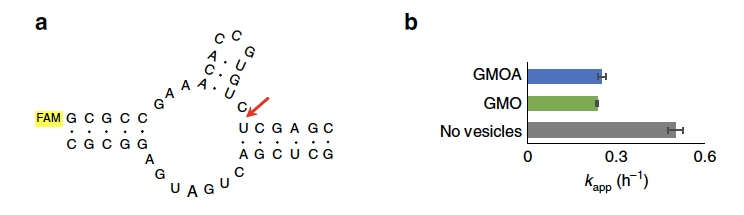
\includegraphics[width=0.9\textwidth]{ProtocellsAndReactions3}
\end{figure}



See \cite{adamala2016programmable} and \cite{monnard2015current}.

See movie, where we see growing vesicle stealing material from neighbour. 
Figure \ref{fig:ProtocellGrowthDivision} illustrates Protocell Growth and division.  

\begin{figure}[H]
	\caption{Protocell Growth and division}\label{fig:ProtocellGrowthDivision}
	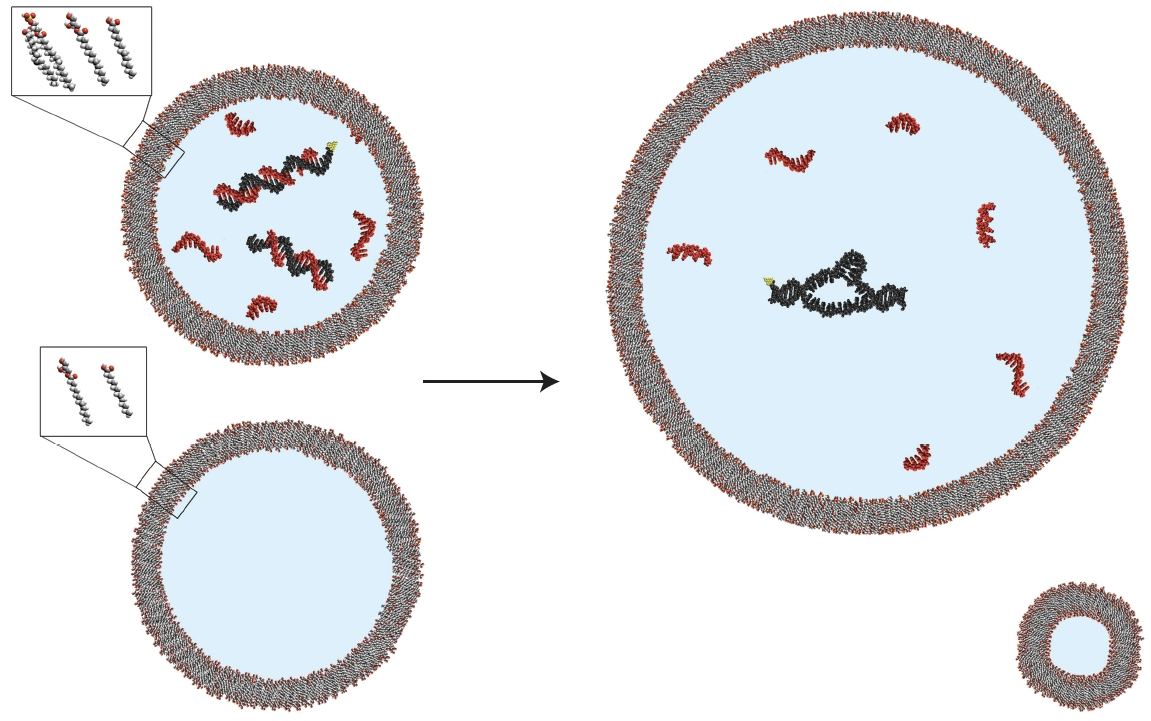
\includegraphics[width=0.9\textwidth]{ProtocellGrowthDivision}
\end{figure}

See  \cite{zhu2012photochemically} and   \cite{chen2004emergence}.

In Figure \ref{fig:TowardsLUCA} we see a prebiotic soup, aggregating, decreasing molecular diversity and increasing functional complexity, and moving towards first life. First life can undergo Darwinian evolution towards \gls{gls:LUCA}.
\begin{figure}[H]
	\caption{Towards LUCA}\label{fig:TowardsLUCA}
	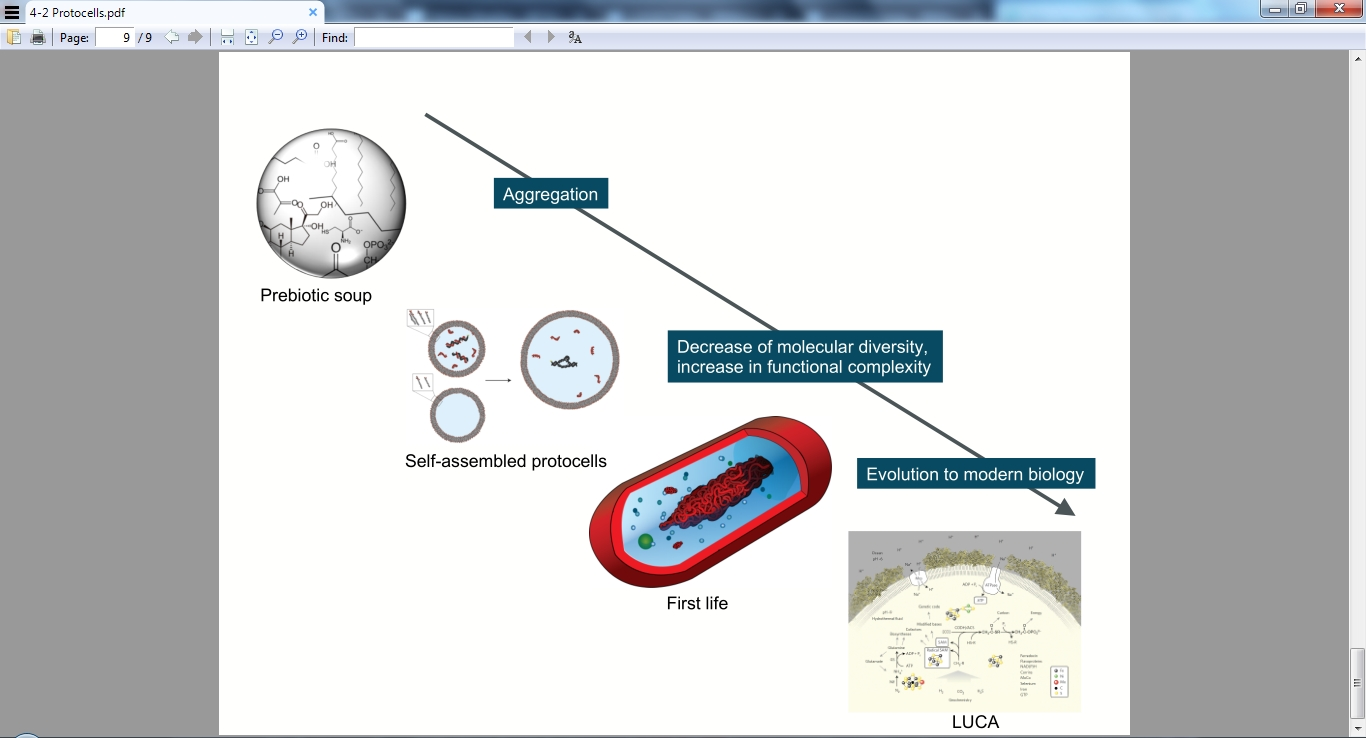
\includegraphics[width=0.9\textwidth]{TowardsLUCA}
\end{figure}

\section{LUCA}

Lecturer: Kate Adamala

Kate discusses the Last Universal Common Ancestor of all Life.

The modern Tree of Life--Figure \ref{fig:TOL4}-- is very diverse in physiology, morphology, and life strategies. But all the diversity  comes from one single ancestor--Figure \ref{fig:TOL_root}.
\begin{figure}[H]
	\caption{The modern Tree of Life}\label{fig:TOL4}
	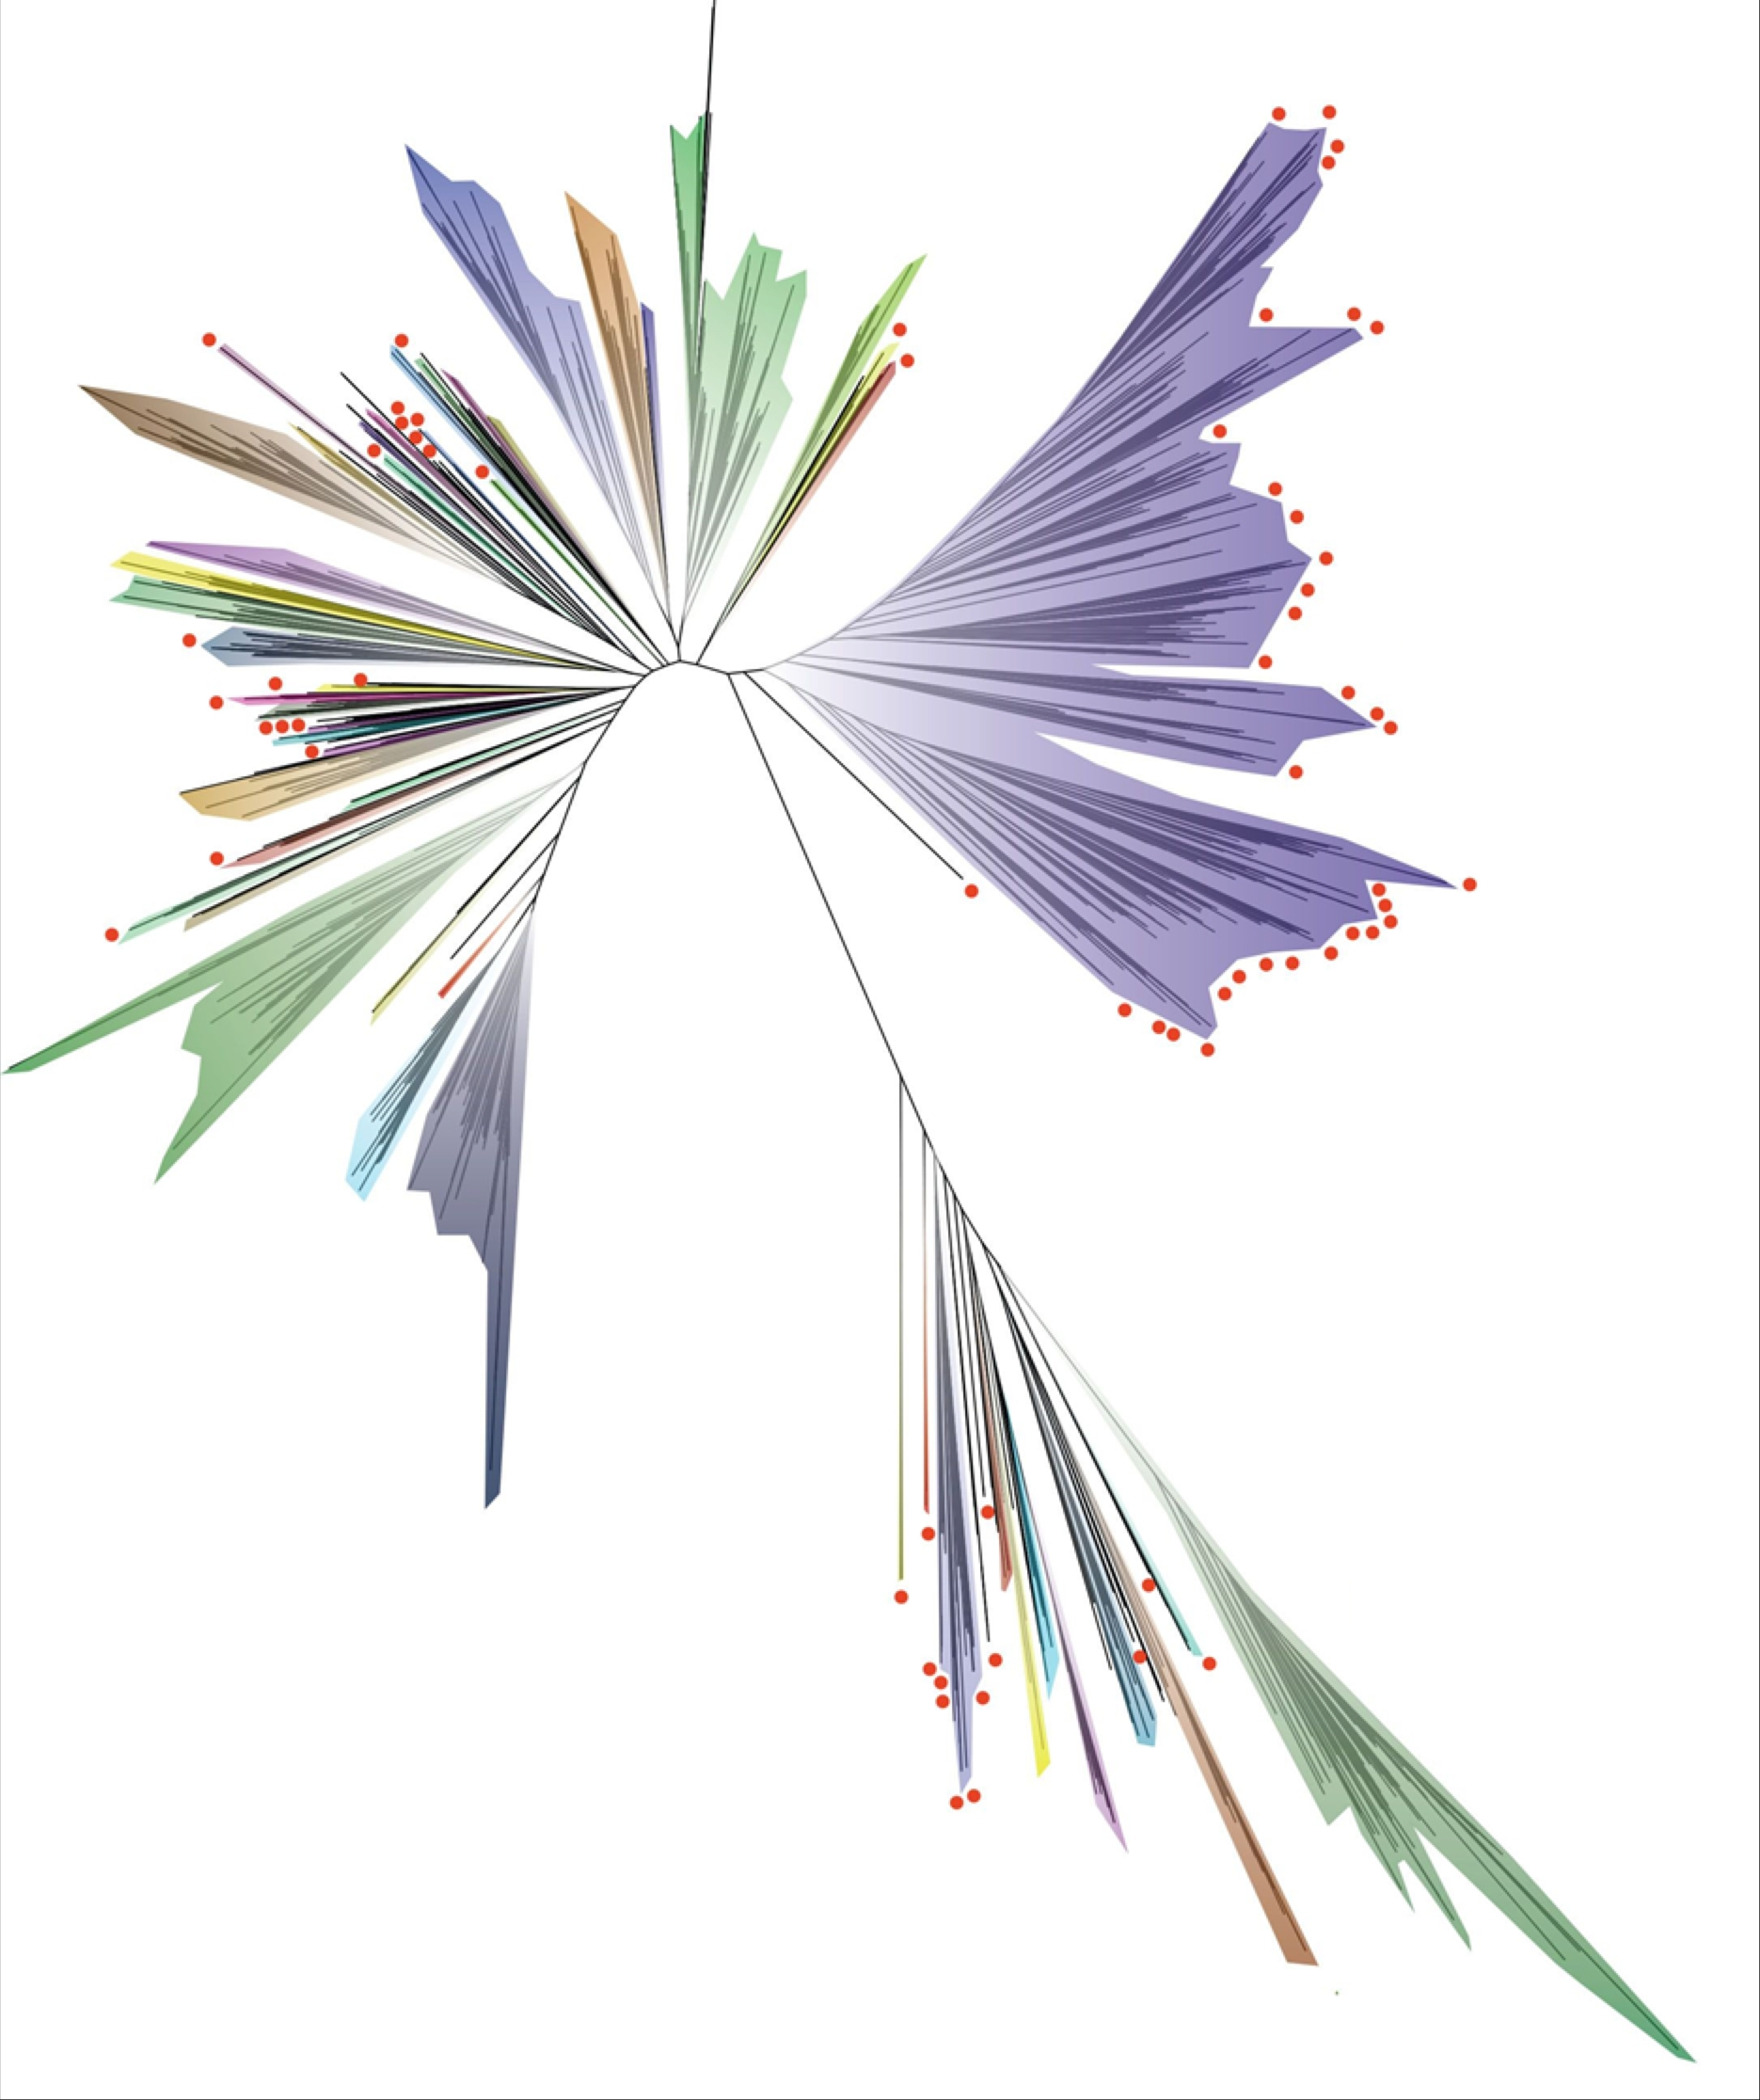
\includegraphics[width=0.9\textwidth]{TOL4}
\end{figure}

\begin{figure}[H]
	\caption{All the diversity of Figure \ref{fig:TOL4} comes from one single ancestor.}\label{fig:TOL_root}
	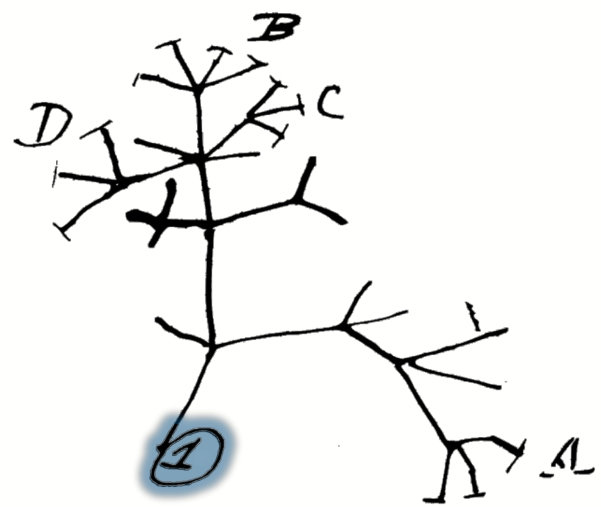
\includegraphics[width=0.9\textwidth]{TOL_root}
\end{figure}

We know that all life came from one population of earliest cells; we know this because all modern life is built on the same principles--Figure \ref{fig:ModernCell}. At one stage, all of life went through the stage of a very simple cell, \gls{gls:LUCA}--Figure \ref{fig:EvolCell}.

\begin{figure}[H]
	\caption{All life came from one population of earliest cells}\label{fig:ModernCell}
	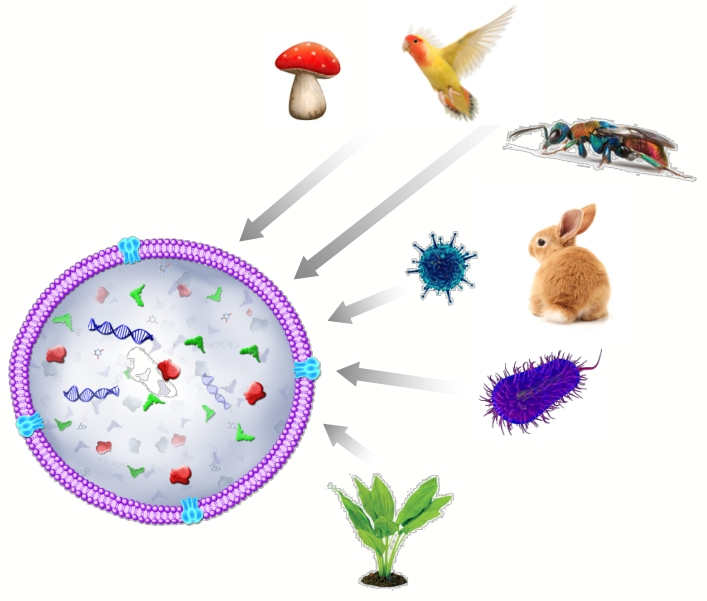
\includegraphics[width=0.9\textwidth]{ModernCell}
\end{figure}

\begin{figure}[H]
	\caption{Evolution of Life, showing very simple cell, LUCA}\label{fig:EvolCell}
	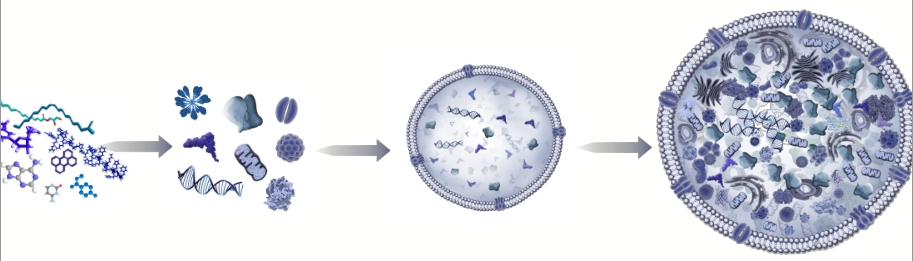
\includegraphics[width=0.9\textwidth]{EvolCell}
\end{figure}

\gls{gls:LUCA} was the ancestor to all modern cells, so it must have possessed the basic mechanisms of  modern cells.

\begin{figure}[H]
	\caption{LUCA must have possessed the basic mechanisms of  modern cells}\label{fig:LUCA_Attributes}
	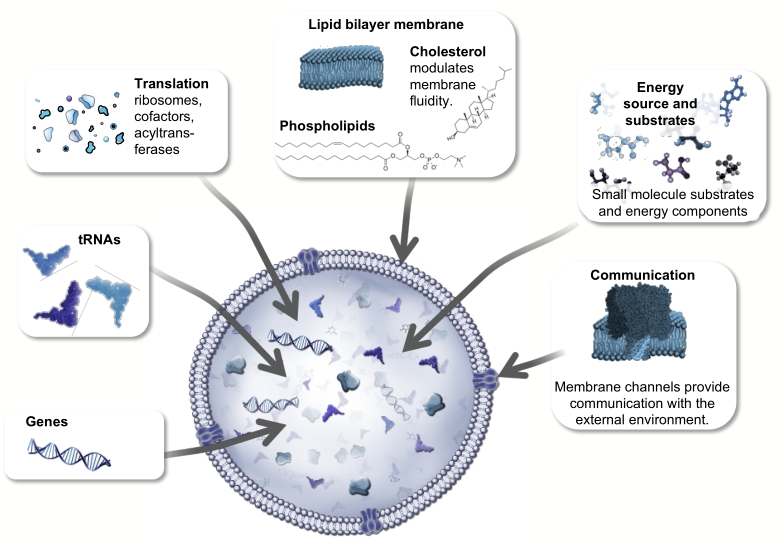
\includegraphics[width=0.9\textwidth]{LUCA_Attributes}
\end{figure}

We know quite a lot about LUCA, but much is still unknown. We can deduce much by studying biochemical evolution and thr properties of modern cells to see what they share.

References:
\begin{itemize}
	\item \cite{penny1999nature}--cytology of PUCA;
	\item \cite{weiss2016physiology}--phylogenomic analysis to determine genome of LUCA;
	\item \cite{torino2013piecing}--reconstruct LUCA in ther lab.
\end{itemize}

\section{Chemical signatures for identifying life in the geological record }

See \cite{sharp2017principles}, \cite{bell2015potentially}, \cite{rosing199913c}, \cite{ueno2006evidence}, \cite{shen2001isotopic}, \cite{summons19992}, \cite{han1992megascopic}

\section{RNA}

\subsection{The RNA World}
\cite{robertson2012origins}, \cite{joyce2018protocells}, \cite{hud2018searching},  \cite{hoshika2019hachimoji}

\subsection{Molecular Evolution in the Lab}

\cite{joyce2007forty}, \cite{seelig2007selection}, \cite{chen2007ribozyme}, \cite{gold2012aptamers}, \cite{sefah2014vitro}, \cite{pinheiro2012synthetic}, \cite{mansy2007structure}, \cite{bartel1993isolation}, \cite{petrie2014limits}, \cite{pressman2019mapping}

\section{Autocatalysis}

\subsection{Autocatalytic Sets: A Cooperative Origin of Life}
\cite{wim2017origin}, \cite{hordijk2017chasing}, \cite{wim2019wandering}, \cite{patzke2007self}, \cite{vaidya2012spontaneous}, \cite{ashkenasy2004design}, \cite{hordijk2012structure}, \cite{sousa2015autocatalytic}

\subsection{Reaction Networks and Autocatalysis}

\section{Evolutionary Theory}

\subsection{An Introduction}

\subsection{A Recipe for Adaptation}

\subsection{Chance \& Change}

\section{Niche Construction}

% end of text 

% glossary
\printglossaries

% bibliography go here
 
\bibliographystyle{unsrt}
\addcontentsline{toc}{section}{Bibliography}
\bibliography{origins}

\end{document}
